\documentclass[]{article}

\usepackage{tikzit}
\usepackage{amsmath}
\usepackage{amsfonts}
\usepackage{mathtools}
\usepackage{amssymb}
\usepackage{hyperref}
\usepackage{physics}
\usepackage{geometry}
\usepackage{blochsphere}
\newcommand{\equaltext}[1]{\ensuremath{\stackrel{\text{#1}}{=}}}


\input{computation.tikzdefs}
\input{computation.tikzstyles}


%opening
\title{}
\author{}

\begin{document}

\maketitle

\begin{abstract}

\end{abstract}

\section{Introduction}

Here I will put the proposal with some adjustments to make it fit in the context of this document.

\section{Preliminaries}

This section serves as a concise introduction to the diagrammatic method for a reader who is familiar with quantum mechanics and Dirac notation. Appendix \ref{Keywords} contains all of the concepts discussed in this section as keywords with hyperrefs to the respective sections.

\subsection{From Dirac to Diagrams}

\subsubsection{States, Effects, and Hermitian Operations}

\label{braandket}
The \textbf{ket} is defined as a triangle with its sharp edge down in diagrammatic notation. It can be interpreted as the preparation of a state, in this case $\psi$. It is referred to as \textbf{state} throughout the thesis.

\begin{equation}
\label{equation:state}
\ket{\psi} =  \tikzfig{state}
\end{equation}

The \textbf{bra} in diagrammatic notation is the flipped state, and is referred to as \textbf{effect}. 

\begin{equation}
\label{equation:effect}
\bra{\psi} =  \tikzfig{effect}
\end{equation}

Triangles are the smallest building blocks in the diagrammatic notation. Most diagrams can be reduced to just triangles. This makes them a powerful tool for translating complicated diagrams to Dirac notation and vice versa.

From the fact that the \textbf{Hermitian adjoint} of a bra gives a ket and reversedly it follows that the operation of flipping a diagram around its horizontal axis corresponds to taking the Hermitian adjoint diagrammatically. Flipping a diagram around its vertical axis is also a legal operation and this corresponds to taking the \textbf{Hermitian conjugate}. Both of these operation applied together takes the \textbf{transpose}. All of these diagram operations can be summarized as follows:

\begin{equation}
\tikzfig{operationssummary}
\end{equation}

Equations \ref{equation:state} and \ref{equation:effect} show the most general method of writing a bra and a ket in diagrammatic notation. However, the notation also allows for us to take these states and effects further apart. For the state this goes as follows: 

\begin{equation}
\label{effectapart}
\begin{pmatrix}
\psi_0 \\
\psi_1 \\
\vdots \\
\psi_n
\end{pmatrix} = \tikzfig{state} = \sum\limits_{i=0}^{n} \psi_i \tikzfig{wiretrianglenosum}
\end{equation}

The effect is then simply the adjoint of equation \ref{effectapart}. Note that the triangle in this equation is not on its side. This is because it is an integer, which is independent of conjugate transformations. 

\subsubsection{Wires}
\label{identity}
The identity map in the diagrammatic notation is given by the following diagram, referred to as a \textbf{wire}.

\begin{equation}
\tikzfig{wire}
\end{equation}

A wire can be reduced to triangles (and subsequently to a ket and a bra) as follows: 

\begin{equation}
\label{equation:wiredecomposed}
\tikzfig{wire} = \tikzfig{wiretriangles} = \sum_{i}\ket{i}\bra{i}
\end{equation}

Every wire has an associated \textbf{system type}, the space of the information that it carries. In the context of this report, the system types are Hilbert spaces or the tensor product of Hilbert Spaces. The latter being the result of the horizontal composition of two wires where each wire has a Hilbert space as system type. This follows from the fact that the horizontal composition of two diagrammatic components is the tensor product of those components in diagrammatic notation. More explanation on this is given in section \ref{doubling}.

\subsubsection{Maps}
\label{maps}

A \textbf{linear map} is given by the following diagram:

\begin{equation}
\tikzfig{map}
\end{equation}

We can find the equivalent form in Dirac notation as follows:

\begin{equation}
\tikzfig{map} = \tikzfig{mapdecomposition} = \sum_{ij}r_{ij}\ket{i}\bra{j}
\end{equation}

In the context of a bra and a ket, we can translate the diagrammatic linear map to Dirac notation as such:

\begin{equation}
\tikzfig{mapincontext} = \bra{\psi}f\ket{\phi}
\end{equation}

\subsubsection{Spiders}
\label{spiders}

A \textbf{spider} is a special map which functions as a Kronecker delta. It forces the inputs to be the same as the outputs. In the case where we have one input and output this gives a trivial result:

\begin{equation}
\tikzfig{spider} = \tikzfig{wiretriangles} = \tikzfig{wire}
\end{equation}

In the case where there are multiple outputs and inputs it forces all to be the same \footnote{Note that this is the first time we have placed diagrammatic components side by side. This can be interpreted as taking the tensor product over those components. We will work this out further in section \ref{doubling}}:

\begin{equation}
\label{equation:spidermultilegdecomposed}
\tikzfig{spidermultileg} = \tikzfig{spidermultilegdecomposed}
\end{equation}

By applying arbitrary in- and outputs we can see how the \textbf{Kronecker delta} arises from Dirac notation. The following example is for two two inputs and two outputs but the same principle extends to an arbitrary amount of in- and outputs.

\begin{equation}
\begin{split}
\tikzfig{spidermultileginandoutputs} = \tikzfig{spidermultilegdecomposedinandoutputs} = \\ \sum_{i} \bra{i}\ket{j}\bra{i}\ket{k}\bra{l}\ket{i}\bra{m}\ket{i} = \delta_{jk} \delta_{lm}  \delta_{jl}
\end{split}
\end{equation}

Spiders with single in- or outputs also exist. A spider with a single input is the deletion of a classical variable and a spider with a single output is the creation of a random classical variable:

\begin{equation}
\tikzfig{spideroneoutput} = \tikzfig{wiretriangle} = \ket{0} + \ket{1}
\end{equation}

An important property of spiders is that they fuse:

\begin{equation}
\label{equation:spiderfusion}
	\tikzfig{spidermultileg2} = \tikzfig{spidermultileg1.1}
\end{equation}

\subsubsection{Phase Spiders}
\label{phasespiders}

\textbf{Phase spiders} follow the same rules as normal spiders. However, perhaps unsurprisingly, they carry a \textbf{phase}. This phase is subject to a new set of rules which is evident from the definition of the phase spider. 

\begin{equation}
\label{phasespider}
\tikzfig{spidermultilegphase} = \tikzfig{spidermultilegdecomposedphase}
\end{equation}

When two phase spiders meet, they fuse like normal spiders and their phases add:
\begin{equation}
	\tikzfig{spidermultileg2phase} = \tikzfig{spidermultileg2phase2} =\tikzfig{spidermultileg11phase0} =\tikzfig{spidermultileg11phase}
\end{equation}


Furthermore, note that since complex phases get flipped in conjugate transformations, the conjugate of a spider is that same spider with an inverted phase:

\begin{equation}
\tikzfig{ConjugateSpider}^* = \sum\limits_{i}(e^{i\alpha_i})^*= \sum\limits_{i}e^{-i\alpha_i} = \tikzfig{conjugatespider1}
\end{equation}

\subsubsection{Colors and Bases}
\label{coloursandbases}

In the diagrammatic notation, the \textbf{color} of an object such as a spider or a triangle determines its basis. For now, we will define two orthonormal \textbf{bases}, the Z and X bases. Later on, as more bases will be necessary they will be introduced accordingly. The Z basis has white diagrammatic elements and for the X basis they are gray. The following is an example of how to translate between bases in this notation:

\begin{equation}
\tikzfig{gray0} =\frac{1}{\sqrt(2)}( \tikzfig{white0} + \tikzfig{white1})
\end{equation}

\begin{equation}
\tikzfig{gray1} =\frac{1}{\sqrt(2)}( \tikzfig{white0} - \tikzfig{white1})
\end{equation}

This equation is of course entirely analogous to its Dirac notation counterpart, with $\ket{-}$ and $\ket{+}$ being the orthonormal basis states in the X basis and $\ket{0}$ and $\ket{1}$ the orthonormal basis states in the Z basis:

\begin{equation}
\ket{\pm} = \frac{1}{\sqrt{2}}(\ket{0} \mp \ket{1})
\end{equation}

Note that spiders of different colors do not fuse.

\subsubsection{Doubling}
\label{doubling}

\textbf{Doubling} is the operation of taking the \textbf{tensor product} of a diagram with itself. In the usual case, where the system type of a single wire is a Hilbert space ($\mathcal{H}$), the doubled wire has the set of density matrices on that Hilbert space as system type.:

\begin{equation}
\mathcal{H} \otimes \mathcal{H} \cong \mathcal{D}(\mathcal{H})
\end{equation}
\textit{Where $\mathcal{D}(\mathcal{H})$ is the set of density matrices on $\mathcal{H}$. $\otimes$ is the tensor product.}

Doubled maps and and states represent \textbf{pure} maps and states. Single maps and states represent their \textbf{mixed} counterparts. The most intuitive interpretation, and how it is mostly used in this report, is that the single wires represent classical data and thick wires represent data encoded into a quantum state.

Doubling in diagrammatic notation is nothing more than placing a second conjugate diagram next to the original diagram. In doubled diagrams lines are drawn thick, a doubled state is thus represented as follows:

\begin{equation}
	\tikzfig{DoubleStateDecomposed} = \tikzfig{DoubleStateDecomposed1}
\end{equation}
\textit{The notation of a state with a hat, such as $\hat{\psi}$, means that that state is pure.}

Taking this further apart, we can define an arbitrary density matrix as follows:

\begin{equation}
	 \sum\limits_{ij} \rho_{ij} \tikzfig{wiretrianglenosum} \tikzfig{wiretrianglenosumj} = \tikzfig{DensityState}
\end{equation}

Note that in te case of doubled states, effects, or maps with multiple in- or outputs we need to make sure that the single wires converge correctly:

\begin{equation}
\tikzfig{conjugatemaps} = \tikzfig{doublemap}
\end{equation}
\textit{The notation of a map with a hat, such as $\hat{f}$, means that that map is pure.}

Doubled spiders among themselves follow the same rules as normal spiders. That is, they follow the fusion rule from equation \ref{equation:spiderfusion}. However, when a single and double spider meet, they fuse to form one single spider, a so called bastard spider. In diagrams:

\begin{equation}
	\tikzfig{BastardSpiderFusion} = \tikzfig{BastardSpiderFusion2}
\end{equation}

\subsubsection{Discarding}
\label{discarding}

\textbf{Discarding} is the process of removing part of a diagram from the whole, or removing the whole diagram altogether. For doubled diagrams it is defined as follows:

\begin{equation}
\label{discarding}
\tikzfig{Discarding} = \tikzfig{thickwhiteieffect} = \tikzfig{thinwirediscardingdecomposed} = \tikzfig{discardingsinglewires} 
\end{equation}

It is trivial to see that applying discarding to any arbitrary (normalized) state always results in the number 1. In fact, discarding a state or map is equivalent to taking its \textbf{trace}. As an example, we discard an arbitrary normalized \textbf{density matrix}, $\rho$:

\begin{equation}
\label{equation:discarding}
\begin{split}
\tikzfig{discardingdensitymatrx} = \tikzfig{discradingdensitymatrixsinglewires} = \sum\limits_{ij} \rho_{ij} \bra{j}\ket{i} \\ = \sum\limits_{ii} \rho_{ii} = Tr(\rho) = 1
\end{split}
\end{equation}

Discarding is not a pure map. It connects the two counterparts of a doubled state by a single wire. This allows for discarding to be used to purify any arbitrary state or map. For the case of a map $\Phi$, \textbf{purification} is as follows:

\begin{equation}
\label{equation:Purification}
\tikzfig{doublemapnotpure} = \tikzfig{doublemapdiscardingoneout} = \tikzfig{conjugatemapsdiscardingoneout}
\end{equation}

Taking the conjugate of the discarding map is actually the preparation of the fully mixed state up to some constant:

\begin{equation}
	\tikzfig{FullyMixed} = \sum\limits_{i=0}^n \tikzfig{Encoding3} \approx \sum\limits_{i=0}^n \frac{1}{n} \ket{i} \bra{i}
\end{equation}

\subsubsection{Entanglement}
\label{entanglement}
Pure entangled states are those states that are not horizontally separable: 

\begin{equation}
\tikzfig{WideStateTwoOutputs} \neq \tikzfig{TwoStates}
\end{equation}

Since horizontally composed states form the \hyperref[doubling]{tensor product} of those states diagrammatically, this definition is in line with theory, where entangled states are defined as those states that can not be written as the tensor product of two states \cite{nielsen2011}. 

An example of such a state is the following:

\begin{equation}
\tikzfig{DoubleCup} = \sum\limits_{i} \tikzfig{DoubleCupSeperate} = \ket{00} + \ket{11}
\end{equation}

Which is up to a number the first Bell state, $B_0$. Although it may seem like this state separates since it is made up of two triangles, it does not. Both triangles are correlated through the same index. Indeed, if the indices were different for each of the triangles this would not be an entangled state.

\subsection{Advanced diagrammatic concepts}

\subsubsection{The yanking equations}

In \cite{Coecke2017} the authors introduce a couple of equations for bending around wires called the yanking equations. One of them will be used later on in this report, so it will be introduced here:

\begin{equation}
	\label{equation:yankingequation}
	\tikzfig{YankingEquations1} = \tikzfig{wire}
\end{equation}

We can easily check that this is true by decomposing the wires to triangles as follows:

\begin{equation}
	\tikzfig{YankingEquations1} \equaltext{\ref{equation:wiredecomposed}} \sum\limits_{ij} \tikzfig{YankingEquations2} = \sum\limits_{ij} \delta_{ij} \tikzfig{YankingEquations3} = \sum\limits_{i} \tikzfig{wiretriangles1} \equaltext{\ref{equation:wiredecomposed}} \tikzfig{wire}
\end{equation}

\subsubsection{Basis and phase translations on the Bloch sphere}

In section \ref{coloursandbases} we already saw how to translate between different bases diagrammatically. The approach was to translate Dirac bra's and kets directly to the appropriate triangles. Using phase spiders, we can employ a more purely diagrammatic method. This stems from the fact that applying a phase to a state corresponds to a rotation on the Bloch sphere. Let's see where a spider without a phase lies on the Bloch sphere:

\begin{equation}
\tikzfig{spideroneoutput} = \tikzfig{wiretriangle} = \tikzfig{white0} + \tikzfig{white1} \approx \frac{1}{\sqrt{2}}(\tikzfig{white0} + \tikzfig{white1}) = \tikzfig{gray0}
\end{equation}

On the Bloch sphere in equation \ref{equation:blochsphere} we indeed see that the phaseless white spider is on the same location as the gray state 0.

For a white spider with a phase of $\pi$ we get the following:

\begin{equation}
\tikzfig{spideroneoutputpiphase} = \sum\limits_{i} e^{i\alpha_i}\tikzfig{wiretrianglenosum} = e^{0}\tikzfig{white0} + e^{i\pi}\tikzfig{white1} \approx \frac{1}{\sqrt{2}}(\tikzfig{white0} - \tikzfig{white1}) = \tikzfig{gray1}
\end{equation}

So a white spider with $\pi$ phase corresponds to the gray state 1. 

The gray spiders and white basis have a similar relationship and these are included as well in equation \ref{equation:blochsphere}.

\label{basisandphasetranslations}
\begin{center}
\begin{equation}
\label{equation:blochsphere}
\begin{blochsphere}[radius=5 cm,tilt=10,rotation=0.01, opacity=0]
	\centering
	%\drawBallGrid[style={opacity=0.3}]{30}{30}

	\drawGreatCircle[]{90}{90}{0}
	\drawGreatCircle[style=dashed]{0}{0}{0}

	\labelLatLon{up}{90}{0};
	\drawStateLatLon[tilt=0.1]{up}{0}{0}
	%\labelLatLon{down}{-90}{90};
	
	\labelLatLon{up}{-90}{90};
	\drawStateLatLon[tilt=0.1]{up}{-10}{100}
	
	\labelLatLon{up}{90}{-90};
	\drawStateLatLon[tilt=0.1]{down}{90}{90}
	
	\draw (4, 1.0) node[anchor=north west] {$\mathbf {\hat{x}}$};
	%\drawStateLatLon[tilt=90]{up}{30}{45}
	\draw (-0.8,4.5) node[anchor=north west] {$\mathbf {\hat{z}}$};
	% Above node
	\draw (-1.8,0.2) node[anchor=north west] {$\mathbf {-\hat{y}}$};
	% Above node
	\node[above] at (0,5.5cm) { $\approx$ };
	\node [style=StateMid] (0) at (-1.3,6.5cm) {\rotatebox{135}{0}};
	\node [style=GraySpider] (0) at (1.2,5.9cm) {0};
	
	% Bottom node
	\node[below] at (0,-5.5cm) {{ $\approx$ }};
	\node [style=StateMid] (0) at (-1.3,-5.3cm) {\rotatebox{-45}{1}};
	\node [style=GraySpider] (0) at (1.2,-5.8cm) {$\pi$};
	
	% Right node
	\node[below] at (7.8,0) {{ $\approx$ }};
	\node [style=StateMidGray] (0) at (6.5,0.3cm) {\rotatebox{-45}{0}};
	\node [style=WhiteSpider] (0) at (8.7,-0.2cm) {0};
	
	% Left node
	\node[below] at (-7.0,0) {{ $\approx$ }};
	\node [style=StateMidGray] (0) at (-8.2,0.3cm) {\rotatebox{-45}{1}};
	\node [style=WhiteSpider] (0) at (-6.1,-0.2cm) {$\pi$};
	
\end{blochsphere}
\end{equation}
\end{center}
\subsubsection{Encoding and Decoding}
\label{encodingdecoding}

Diagrammatically, the encoding map is a single spider with one doubled wire as output and one single wire as input. The color of the spider is the basis in which the classical bit gets encoded into a quantum state. For example, encoding classical information $p$ on a diagonal density matrix $\rho$ into a quantum state in the white basis with indices $i \in \{0,1\}^n$:

\begin{equation}
	\label{equation:Encoding}
	\tikzfig{Encoding} = \sum\limits_{i} \tikzfig{Encoding2} = \sum\limits_{i} \bra{p}\ket{i} \tikzfig{Encoding3} = \tikzfig{DensityState}
\end{equation}

The decoding map is the adjoint of the encoding map. Its behavior follows directly from (\ref{equation:Encoding}).

Phases get lost when decoding quantum states to classical states. We can rely on our knowledge of phase spiders to see how the phase gets eliminated in the process of \textbf{decoding} a quantum state with a phase $ \alpha$ to classical information.

\begin{equation}
\label{eq:20}
\tikzfig{decodingphase} = \tikzfig{spidertwophases} = \tikzfig{spidertwophaseswrittenout} = \tikzfig{spideronephasefromtwo} = \tikzfig{spideronephasefromtwoinspider} =
\tikzfig{uniformprobstate}
\end{equation}

\subsubsection{Complementary spiders}
\label{complementarity}
Alice encoding a classical state into a qubit in a certain basis and then Bob measuring that qubit in a complementary basis results in Bob receiving a random bit.


\begin{equation}
	\label{equation:Complementarity}
	\tikzfig{ComplementarySpiders} = \tikzfig{ComplementarySpiders2}
\end{equation}

\subsubsection{The xor map}

\label{xorgate}

The Exclusive OR (xor) map takes two inputs and gives an output of 0 when the inputs are the same and 1 when they are different. Mathematically, if we take $x, y \in \{0,1\} $ as inputs the output of the xor gate is $(x + y)~mod~2$. We could just define a diagrammatic map and give it this property. However, there is another way of creating the xor map diagrammatically which only uses spiders. This has the advantage of allowing us to use spider rules to move xor maps around in diagrams.

If we enter two outputs of a certain basis into a spider that is of another basis orthonormal to the inputs this gives the xor map. To see how this works, let's use a gray spider and apply white test in- and outputs. First, recall that:

\begin{equation}
	\tikzfig{XORProof1} \equaltext{\ref{coloursandbases}} 1/\sqrt{2} ~~~~~~~~~~~~~~~~~ \tikzfig{XORProof2} = (-1)^i/\sqrt{2}
\end{equation}

Now applying the test in- and outputs to the proposed xor map \cite{Coecke2017}:

\begin{equation}
	\label{equation:xormap}
	\tikzfig{XORTestInAndOutputs} \equaltext{\ref{spiders}} \tikzfig{XORTestInAndOutputs1} + \tikzfig{XORTestInAndOutPuts2} = \frac{1}{\sqrt{2}} * \frac{1}{2}(1+(-1)^{i+j+k})
\end{equation}

This equation results in 0 whenever the sum $i+j+k$ is uneven and 1/$\sqrt{2}$ when it is even. Now $i+j+k$ is only even whenever $i \oplus j = k$. This thus, up to a factor of $\sqrt{2}$, gives the xor map.

\subsubsection{The essential uniqueness of purification}
\label{section:essentialuniqueness}

The essential uniqueness of purification is a theorem that states the following: Given two pure maps $\hat{V}_1$ and $\hat{V}_2$ that satisfy $V_1$, $V_2$: $\mathcal{H}$ $\rightarrow$ $\mathcal{L}$ $\otimes$ $\mathcal{K}$ and:

\begin{equation}
	\label{equation:uniquenesspurification}
	\tikzfig{Vhat1purifiedX} = \tikzfig{Vhat2purifiedX}
\end{equation}

Then there exists some unitary $U$: $\mathcal{L}$ $\rightarrow$ $\mathcal{L}$ such that:

\begin{equation}
	\tikzfig{VunpurifiedX} = \tikzfig{V2unpurifiedX}
\end{equation}

Intuitively, this theorem states that if $\hat{V}_1$ and $\hat{V}_2$ are similar to the extent that they satisfy equation (\ref{equation:uniquenesspurification}), then the linear maps $V_1$ and $V_2$ can only differ by some unitary U. This is an adaptation of the theorem given by Kissinger and Westerbaan in section 2.1 of \cite{Kissinger2017} that is better suited to this report.

Note that whereas here $\hat{V}_1$ and $\hat{V}_2$ have two output wires that are discarded, this theorem scales for maps with an arbitrary number of outputs. In other words, $\mathcal{L}$ could be the Hilbert space of a composite system.

\subsubsection{The $k-k'$ commute rule}
\label{section:kkcommute}
In this report we will on multiple occasions want to move certain phase spiders past one another. This does, however, require some more advanced diagrammatic derivations that are too extensive for the scope of this report. Therefore we show the result here, and refer to the relevant literature. In \cite{Coecke2017} on page 771, Coecke and Kissinger introduce the $k-k'$ commute rule and give the full diagrammatic derivation to arrive to this rule. As we will later see, this rule is the main ingredient for pushing Pauli's past one another diagrammatically. It states that for $k, k' \in \{0, \pi\}$: 

\begin{equation}
\label{equation:kkcommuterule}
\tikzfig{kkcommuterule} = \tikzfig{kkcommuterule1}
\end{equation}

This rule shows us how we can move phase spiders of a different color with either a $\pi$ or no phase past one another.

\section{Protocols}


\subsection{One Time Pad}

The classical One Time Pad (OTP) is perhaps the oldest and most well known cryptographic method. We will first discuss this protocol as a setup to the quantum version. Although originally proposed in 1884 \cite{Markoff2011}, the OTP was first formalized and proven secure in 1949 \cite{Shannon1949}. Since then, the scheme has essentially remained the same due to its simplicity. A typical OTP goes as follows:

Alice and Bob start with a uniformly random key $k \in \{0,1\}^n$. Alice wants to send some message $m \in \{0,1\}^n$ to Bob. She encrypts $m$ using the key $k$ by means of an xor map, generating ciphertext $x^n = m \oplus k$.\footnote{In different realizations of the OTP, Alice has different methods of encrypting her message. With that being said, applying an xor to the key and the message is one of the most common versions.} After this step, she sends $x$ to Bob who applies $k$ again to $x$ to receive $m$ since $k \oplus x = m$. The assumption on Eve in this scheme is that she doesn't know $k$ and can intercept $x$. With that being said, if $k$ was truly uniformly random, $x$ is so too, leaving Eve with a random variable even after a successful interception. The main drawback of this scheme is the fact that the key has to be the same size as the message and that this key can only safely be used once.

\subsubsection{Diagrammatic Representation}

The OTP relies on classical communication channels and xor gates. Since we can represent both of these diagrammatically we can draw out the fully classical OTP protocol by means of diagrams. Recall from section \ref{spiders} that the following state generates a random bit:

\begin{equation}
	\tikzfig{spideroneoutput}
\end{equation}

We choose this as the uniformly random key $k$ and give one copy to Alice and one to Bob. Alice, who starts with message $m$, then applies the xor gate from section \ref{xorgate} to this message, generating ciphertext $x$:

\begin{equation}
	\tikzfig{OTPProof1}
\end{equation}
\textit{Note that the dotted line used here is only to illustrate what part of the diagram and Alice "control" and that it bears no physical significance.}
Everything Bob now has to do is to apply an xor gate to the ciphertext $x$ and the key $k$:

\begin{equation}
\label{equation:OTPProof2}
\tikzfig{OTPProof2}
\end{equation}

To check that this is indeed a viable communication protocol we want equation (\ref{equation:OTPProof2}) to reduce to:

\begin{equation}
\label{equation:OTPProof3}
\tikzfig{OTPProof3}
\end{equation}

This happens up to a constant factor:

\begin{equation}
\label{equation:OTPProoflong}
\tikzfig{OTPProof2}\equaltext{\ref{equation:spiderfusion}} \tikzfig{OTPProof4} \equaltext{\ref{doubling}} \tikzfig{OTPProof5} \equaltext{\ref{equation:Complementarity}} \tikzfig{OTPProof6} \approx \tikzfig{OTPProof7}
\end{equation}

*** Add Eve! ***

\subsection{Quantum One Time Pad}
\label{QOTP}
In the Quantum One Time Pad (QOTP) Alice and Bob share a uniformly random key $ \alpha \in \{0,1,2,3\}^n$ and want to communicate some quantum state, $\rho$. Alice first transforms $\rho$ with a random Pauli map, $\sigma_\alpha$. After she has prepared this state she sends it to Bob over a quantum channel. He can then apply the Hermitian adjoint of this random Pauli resulting in the original $\rho$ sent by Alice. This step exploits the unitary property of the Pauli maps. Eve, who doesn't know $\alpha$, can observe the state sent from Alice to Bob. However, from her perspective, this is the fully mixed state. Mathematically, this can be seen as follows:

\begin{equation}
	\label{equation:OTPsecurity}
	\rho' = \sum\limits_{\alpha = 0}^3 \frac{1}{4} \sigma_\alpha \rho \sigma_\alpha^\dagger = \frac{1}{2}\mathbb{I}
\end{equation}

In principle, the QOTP is similar to the OTP. By means of encrypting a piece of information with a random key which is unknown to Eve but shared by Alice and Bob the latter can achieve secure communication. As a communication protocol, QOTP is not very efficient. Alice and Bob need use two bits as a key per qubit of communicated information.

\subsubsection{Diagrammatic Representation}
\label{DiagramRepresentationQOTP}
In the diagrammatic formalism we can construct a set of maps that have the same property as the Pauli maps in equation \ref{equation:OTPsecurity}, the Bell maps. These are defined in terms of the Pauli matrices as follows \cite{Coecke2017}:

\begin{equation}
	\sigma_0 = B_0 ~~~ \sigma_1 = B_1 ~~~ \sigma_2 = iB_3 ~~~ \sigma_3 = B_2 
\end{equation}
\textit{In the appendix, these Bell matrices are written out. Note that since they have the same properties as Pauli matrices we use them interchangeably throughout the report.}

In order to form diagrams for these Bell maps we have to understand them a little bit better. One of their properties is that they can be constructed from rotations on the Bloch sphere around the z and x axes \cite{DJORDJEVIC2012227}, also known as bitflips around these axes. Note that the maps that apply bitflips are themselves actually Pauli maps. It was chosen to give them their own notation such that they more explicitly represent their behavior. X refers to a bitflip around the x axis and Z refers to a bitflip on the z axis. For random $u, w \in \{0,1\}$ and $\alpha \in \{0,1,2,3\}$ dependent on $u$ and $w$ we can write this mathematically as follows:

\begin{equation}
\label{randombell}
	Z^uX^w = B_{uw} = B_\alpha ~(\text{where}\ \alpha = u + 2w)
\end{equation}
\textit{Where $Z$ and $X$ denote the maps that do a bitflip in the z and x bases respectively. Note that $Z = \sigma_3$ and $X = \sigma_1$.}

Let's see if we can construct these smaller constituents, $Z^u$ and $X^w$, diagrammatically. Starting with $X^w$, remember that a bitflip in the x basis corresponds to a rotation around the z axis on the Bloch sphere. Therefore we need to find a diagrammatic map that either rotates the Bloch sphere around its z axis by $\pi$ radians ($X^1$) or not ($X^0$). Since a single spider without a phase is the identity \ref{spiders} and the z basis is represented by the color white diagrammatically, we can use the white phaseless spider for the case where we don't flip the bit or rotate around the z axis. Let's send the 0 state through in the gray (x) basis to test if this map behaves as expected:

\begin{equation}
	\label{equation:nobitflip}
	\tikzfig{NoBitFlipOnGray0(1)} \equaltext{\ref{coloursandbases}} \frac{1}{2}\tikzfig{NoBitFlipOnGray0(2)} +  \frac{1}{2}\tikzfig{NoBitFlipOnGray0(3)} 
	\equaltext{\ref{spiders}}
	\frac{1}{2}
	\tikzfig{NoBitFlipOnGray0(4)} 
	\equaltext{\ref{phasespiders}}
	\frac{1}{2}
	\tikzfig{NoBitFlipOnGray0(5)} 
	\equaltext{\ref{coloursandbases}}
	\tikzfig{NoBitFlipOnGray0(6)}
\end{equation}

This map does seem to behave appropriately. We see that whenever we send a gray 0 through, we get a gray 0 as output. Following similar logic, we could also use the white spider with a $\pi$ phase to make a rotation around the z axis, and thus a bitflip in the x basis. Let's test if this works too:

\begin{equation}
\label{equation:bitflip}
\tikzfig{BitFlipOnGray0(1)} \equaltext{\ref{coloursandbases}} \frac{1}{2}\tikzfig{BitFlipOnGray0(2)} + \frac{1}{2}\tikzfig{BitFlipOnGray0(3)} 
\equaltext{\ref{spiders}}
\frac{1}{2}
\tikzfig{BitFlipOnGray0(4)} 
\equaltext{\ref{phasespiders}}
\frac{1}{2}
\tikzfig{BitFlipOnGray0(5)} 
\equaltext{\ref{coloursandbases}}
\tikzfig{BitFlipOnGray0(6)}
\end{equation}

These maps do exhibit the correct properties. Indeed, whenever we send a gray 1 through we also get the expected results. It seems that we have formed the $X^0$ and $X^1$ maps. While we will not go through the full math here, the $Z^0$ and $Z^1$ maps follow very similar logic and also behave as expected. Perhaps unsurprisingly, the former is a gray phaseless spider whereas the latter is a gray spider with a phase $\pi$.


Now that we have created our four constituent maps we are in principle ready to make any Bell map of choice. However, we do not want to make a choice, we want to select a random Bell matrix. We still need to find a diagrammatic method to generate a random $u$ and $w$ on which our choice of Bell matrices depend. Recall that generating a random bit is the following diagram: 

\begin{equation}
	\tikzfig{spideroneoutput} \equaltext{\ref{spiders}} \tikzfig{wiretriangle}
\end{equation}

We could encode this random classical bit into a qubit as follows:

\begin{equation}
	\label{eq:7}
	\tikzfig{encodingrandombit} \equaltext{\ref{spiders}} \sum\limits_{i} \tikzfig{encodingrandombit2} \equaltext{\ref{encodingdecoding}} \sum\limits_{i} \tikzfig{IMID}
\end{equation}

The previous two equations are entirely analogous for the gray (x) basis.\footnote{In fact, we can make an even stronger statement about the diagrams in equation \ref{eq:7}: They are actually equal to the analogous diagrams in the gray basis. Note that the rightmost diagram is the adjoint of discarding, which can be interpreted as preparing the fully mixed state, up to a number. Since this state is independent of the basis, these diagrams of white basis are equal to the analogous diagrams in the gray basis.}

We now have the necessary ingredients to make a map that applies a random bitflip or not in x and another map that makes a random bitflip or not in z. The results are as follows:

\begin{equation}
	\label{equation:twodiagrammaticpauli's}
	X^w ~~  \Leftrightarrow ~~ \tikzfig{RandomXBitFlipX} ~~~~~~~~~~~~~~~~~~~~~~~~ Z^u ~~ \Leftrightarrow ~~ \tikzfig{RandomZBitFlipX}
\end{equation}
\textit{Where the gray spider in the $X^w$ map determines the random choice of $w$ and the white spider in $Z^u$ determines the random choice of $u$.}

Let's confirm that the diagrammatic version of $X^w$ does indeed behave as expected:

\begin{equation}
	\label{equation:RandomXBitFlipProof}
	\tikzfig{RandomXBitFlipX} \equaltext{\ref{spiders}}
	\tikzfig{RandomXBitFlipProof(1)X} +
	\tikzfig{RandomXBitFlipProof(2)X} \equaltext{\ref{encodingdecoding}}
	\tikzfig{RandomXBitFlipProof(3)X} +
	\tikzfig{RandomXBitFlipProof(4)X} \equaltext{\ref{basisandphasetranslations}}
	\tikzfig{RandomXBitFlipProof(5)X} +
	\tikzfig{RandomXBitFlipProof(6)X} \equaltext{\ref{phasespiders}}
	\tikzfig{RandomXBitFlipProof(7)} +
	\tikzfig{RandomXBitFlipProof(8)} 
\end{equation}

So depending on whether the random bit was a 0 or a 1, we get the map from equation \ref{equation:nobitflip} ($X^0$) or the map from equation \ref{equation:bitflip} ($X^1$). Again, this derivation is analogous for the map $Z^u$. We have thus successfully made the constituents to our Bell maps. The random Bell map itself is then as follows:

\begin{equation}
	\label{equation:BellMap}
	B_\alpha = Z^uX^w \Leftrightarrow \tikzfig{BellMapX}
\end{equation}

To make a diagrammatic version of QOTP we need to compose the Hermitian adjoint of this Bell map to its input. The bottom Bell map can then be seen as Alice encrypting her state and the top Bell map can be seen as Bob decrypting this state. We also need to make sure that Alice and Bob make the same choice in $\alpha$ and thus use the same Bell map. This can be done by connecting the outputs of the spiders that generate the random numbers to the Bell maps of both Alice and Bob. Furthermore, whereas in the previously described protocol a state $\rho$ is communicated as an example, here we can be more general. We allow the state that Alice wants to communicate to Bob to be any state in any basis. This is represented by a dotted line at the bottom of the diagram. Finally, we need to introduce Eve. She goes in between the Pauli's of Alice and Bob. She can be interpreted as an eavesdropper, but also more generally as the environment. In this sense, Eve could thus also just be a source of noise. She gets the map $\Phi$ that takes as input the state sent by Alice, and outputs one state that she keeps and another that is sent to Bob. In all, this makes QOTP to be the following diagram:

\begin{equation}
\tikzfig{QOTPEveX}
\label{equation:QOTPEve}
\end{equation}

Let us first consider what would happen if there was no noise, and thus no Eve, in the quantum communication channels. Diagrammatically, this looks as follows:

\begin{equation}
	\tikzfig{QOTPNoEveX}
	\label{equation:QOTPNoEve}
\end{equation}

For this protocol to be a good candidate for communication we need equation (\ref{equation:QOTPNoEve}) to reduce to the following: 

\begin{equation}
	\tikzfig{QOTPNoEveFinalX}
\end{equation}

This simply states that Alice's qubit is sent to Bob through the identity map. We already know that this is true due to the unitarity of the Bell maps. Diagrammatically, the proof is as follows:

\begin{equation}
	\begin{split}
	\tikzfig{QOTPNoEveX} \equaltext{\ref{spiders}} 
	\tikzfig{QOTPNoEveProof(1)X} \equaltext{\ref{spiders}}
	\tikzfig{QOTPNoEveProof(2)X} \equaltext{\ref{singleanddoublespiderfusion}}
	\tikzfig{QOTPNoEveProof(3)X} \equaltext{\ref{complementarity}} \\
	\tikzfig{QOTPNoEveProof(4)X} \approx
	\tikzfig{QOTPNoEveProof(5)X} \equaltext{\ref{singleanddoublespiderfusion}}
	\tikzfig{QOTPNoEveProof(6)X} \equaltext{\ref{complementarity}}
	\tikzfig{QOTPNoEveProof(7)X} \approx
	\tikzfig{QOTPNoEveFinalX}
	\end{split}
\end{equation}

Now that we have diagrammatically shown that QOTP without Eve is indeed a communication protocol, we can return to equation (\ref{equation:QOTPEve}) to see what would happen if the protocol did include Eve. First of all, let's see what the result is of Alice encrypting her state by means of a Bell map. To understand what happens in this case diagrammatically we need to first extend equation (\ref{eq:7}). Note that the RHS of this equation is actually the Hermitian adjoint of discarding as it is defined in \ref{discarding}, which is in turn the fully mixed state. Since this state is independent of the choice of basis we can construct the following equation:

\begin{equation}
	\tikzfig{encodingrandombit} = \tikzfig{FullyMixed} = \tikzfig{encodingrandombitgray}
	\label{equation:RandomStateFullyMixed}
\end{equation}

Using equation (\ref{equation:RandomStateFullyMixed}) we can prove that whenever Alice encrypts a state with a Bell map and discards her classical $u$ and $w$ she prepares the fully mixed state:

\begin{equation}
	\label{equation:AliceWithBell}
		\tikzfig{AliceWithBellX} \equaltext{\ref{equation:RandomStateFullyMixed}} \tikzfig{AliceWithBell(1)X} \equaltext{\ref{spiders}} \tikzfig{AliceWithBell(2)X} \equaltext{\ref{singleanddoublespiderfusion}} \tikzfig{AliceWithBell(3)} \equaltext{\ref{complementarity}} 1/D~ \tikzfig{AliceWithBell(4)} \equaltext{\ref{equation:RandomStateFullyMixed}} 1/D~ \tikzfig{AliceWithBell(5)}
\end{equation}
\textit{With D the dimension of the system.}

This might give some intuition for what Eve would receive after Alice has encrypted her state. However, in the full protocol, Alice can not just discard her random $u$ and $w$. Somehow she has to communicate them with Bob. The diagram of QOTP as a communication protocol and Eve with the ability to intercept the quantum state but not $u$ or $w$ is as follows:

\begin{equation}
	\tikzfig{QOTPEveX}
\end{equation}
\textit{Where Eve controls the map $\Phi$ and receives the rightmost output of this map.}

Let's see what happens when we look at this situation from Eve's perspective and thus trace out (discard) Bob's channel.

\begin{equation}
	\label{equation:QOTPEveEvePerspective}
	\tikzfig{QOTPEveEvePerspective(1)X} =
	\tikzfig{QOTPEveEvePerspective(2)X} \equaltext{\ref{equation:RandomStateFullyMixed}}
	\tikzfig{QOTPEveEvePerspective(3)X} \equaltext{\ref{equation:AliceWithBell}}
	\tikzfig{QOTPEveEvePerspective(4)X}
\end{equation}

The third diagram in equation (\ref{equation:QOTPEveEvePerspective}) is up until Eve's map $\Phi$ the same as equation (\ref{equation:AliceWithBell}). We therefore see that from Eve's perspective Alice gives her the fully mixed state due to the Bell map that she applies to her original state. So even in the full protocol, the Bell map is responsible for encrypting the state such that Eve can extract no information from it. 

\subsection{Quantum Teleportation}
\label{subsection:QuantumTeleportation}
In quantum teleportation, Alice and Bob want to communicate a qubit, $\rho_1$, using the fact that they share an EPR pair, $\rho_{23}$, and a classical communication channel. Note that the subscripts in this section help keep track of the different particles present. Subscript 1 refers to Alice's particle, 2 to her side of the EPR pair and 3 to Bob's side of the EPR pair. Alice measures $\rho_1$ together with $\rho_{2}$ in a Bell measurement, entangling these two states to give the total entangled state of $\rho_{123}$. This projects $\rho_{3}$ to one of four possible pure states dependent on the result of the Bell measurement done by Alice. Using the classical communication channel, Alice can send this measurement outcome to Bob in two classical bits. In order for Bob to extract  $\rho_1$ from his part of the entangled state, $\rho_{3}$, he needs to apply to it the Bell map that corresponds to the measurement outcome of Alice's Bell measurement.


The name of this protocol might lead one to think that it includes the teleportation of information. However, this is not the case. This protocol does not achieve faster than light communication. Although the projection of $\rho_{3}$ onto a pure state happens simultaneously with Alice making the Bell measurement, in order for Bob to receive any information on $\rho_1$ from $\rho_{3}$ he must apply the Bell map that corresponds to the measurement result of Alice's Bell measurement. Alice thus has to communicate classically to Bob the result of her Bell measurement.

Quantum teleportation carries some similarity to QOTP. In both protocols, Alice and Bob communicate two classical bits of information in order to communicate one qubit. Also, in both cases, Bob applies a Bell map. These similarities might give some intuition for the equivalence of these protocols. In the end of this section we will see this equivalence diagrammatically.

\subsubsection{Diagrammatic Representation}

The only component of this protocol that we have not worked out diagrammatically yet is the Bell measurement. We know that the Bell measurement is the adjoint of the Bell state. Therefore it suffices to create this Bell state and take its adjoint to make a Bell measurement.

Let's see if we can take the Bell state apart and construct its smaller constituents diagrammatically. The Bell state is actually a composition of a Hadamard (H) and a CNOT gate. The Hadamard gate is applied first to one of the qubits. It transforms $\ket{0}$ to  $(\ket{0} + \ket{1})/\sqrt{2}$ and $\ket{1}$ to $(\ket{0} - \ket{1})/\sqrt{2}$. These superposition states actually form the basis states in a different basis. Therefore, the Hadamard gate can be seen as a basis transformation. For example, a Hadamard gate applied to basis states in the z basis will transform those states to the x basis. The CNOT gate is then applied to the two qubits. In the CNOT gate, one input qubit controls whether or not the other is negated. If the former is $\ket{0}$ the latter undergoes the identity and if the former is $\ket{1}$ the latter is negated. The control qubit in the CNOT gate is in this case the output of the Hadamard gate. The result of these operations entangles the two input qubits and puts them in one of four possible Bell states. Let's test this construction on input state $\ket{00}$ to see if it indeed behaves as expected:

1. The Hadamard gate puts the first qubit in superposition: $\ket{00} \Rightarrow \frac{(\ket{0} + \ket{1})\ket{0}}{\sqrt{2}}$

2. The CNOT negates the second qubit if the first is $\ket{1}$: $\frac{(\ket{0} + \ket{1})\ket{0}}{\sqrt{2}} \Rightarrow \frac{(\ket{00} + \ket{11})}{\sqrt{2}}$

The result is thus indeed one of the Bell states, namely $B_0$.

Diagrammatically, we do not have to construct the whole Hadamard gate to put one of the qubits into the required superposition. In fact, all we have to do is encode one qubit into a different basis than the other and choose one of the two bases to read the results in. The first part of our diagrammatic version of the Bell state thus becomes:

\begin{equation}
	\label{equation:BellState(1)}
	\tikzfig{BellState(1)}
\end{equation}
\textit{Where i and j are test inputs.}

The CNOT gate itself is composed by a copy map and an XOR map. The first qubit is copied after which the second is XOR'd with the copied qubit \cite{articleCNOT}. Diagrammatically:

\begin{equation}
	\label{equation:CNOT}
	\tikzfig{CNOT}
\end{equation}

Applying test states:

\begin{equation}
	\tikzfig{CNOTWithTestInput} \equaltext{\ref{spiders}} \tikzfig{CNOTWithTestInput(1)} \equaltext{\ref{xorgate}} \ket{i} \otimes \ket{i \oplus j}
\end{equation}

Which is indeed the behavior of the CNOT gate.

Composing equations (\ref{equation:BellState(1)}) and (\ref{equation:CNOT}) then gives the Bell state:

\begin{equation}
	\tikzfig{BellState}
\end{equation}

Let's again apply the state $\ket{00}$ to test the functionality of this Bell state preparation map:

\begin{equation}
\label{BellStateTestInput}
	\begin{split}
	\tikzfig{BellStateTestInput} \equaltext{\ref{encodingdecoding}} \tikzfig{BellStateTestInput(1)} \equaltext{\ref{basisandphasetranslations}} \tikzfig{BellStateTestInput(2)} \equaltext{\ref{spiders}} \frac{1}{2}(\tikzfig{BellStateTestInput(3)}) + \frac{1}{2}(\tikzfig{BellStateTestInput(4)}) \\ \equaltext{\ref{spiders}} \frac{1}{2}(\tikzfig{BellStateTestInput(5)}) +
	\frac{1}{2}(\tikzfig{BellStateTestInput(6)}) 
	\equaltext{\ref{basisandphasetranslations}} \frac{1}{2}(\tikzfig{BellStateTestInput(7)}) + \frac{1}{2}(\tikzfig{BellStateTestInput(8)}) \\ \equaltext{\ref{phasespiders}}
	\frac{1}{2}(\tikzfig{BellStateTestInput(10)}) +
	 \frac{1}{2}(\tikzfig{BellStateTestInput(9)}) 
	 \equaltext{\ref{basisandphasetranslations}} \frac{1}{2}(\tikzfig{BellStateTestInput(11)}) +
	\frac{1}{2}(\tikzfig{BellStateTestInput(12)})
	\end{split}
\end{equation}

The result is thus indeed the expected Bell state. Note that whereas usually the constants in the Bell states are $1/\sqrt{2}$ here they are $1/2$ since the final state is doubled.

Let's choose the entangled state of \ref{entanglement} for state $\rho_{23}$. We can then compose the Bell measurement that Alice applies on the left of this entangled state and the Bell map that Bob applies to the right. Alice also inputs $\rho_1$ to the Bell measurement. Using a similar approach to the one we took in \ref{DiagramRepresentationQOTP}, we can generalize this to say that this state can in fact be any quantum state. Again, we can represent this by a dotted line which enters the diagram where $\rho_1$ would go. Finally, we need to make sure to connect the outputs of Alice's Bell measurement to Bob's Bell map. The protocol for teleportation then becomes: 
 
\begin{equation}
	\label{equation:quantumteleportation}
	\tikzfig{QuantumTeleportation}
\end{equation}
 
It is redundant to see what happens to Eve or to show that this protocol allows for communication. This is because we can directly tell that this protocol is equivalent to the QOTP protocol described in section \ref{QOTP}, which was shown to allow for communication without Eve. Placing QOTP without Eve and quantum teleportation side by side, this equivalence is strikingly simple. Everything we have to do is to make a small adjustment to QOTP, writing it a bit more suggestively:

\begin{equation}
\label{equation:QOTPQuantumTeleportationEquivalence}
\tikzfig{QOTPNoEveNoLineX} \equaltext{\ref{spiders}} \tikzfig{QOTPNoEveNoLine(1)}~~~~~ \Leftrightarrow ~~~~~\tikzfig{QuantumTeleportationNoLine}
\end{equation}
 
\subsection{Quantum Key Distribution}

\label{QuantumKeyDistribution}

QKD is the only protocol that has been diagrammatically (somewhat) thoroughly discussed in literature \cite{Kissinger2017}. Therefore, we will not go over the full security proof here. This section is meant to get the reader to understand the diagrammatic version of QKD, such that we can use it later on in the context of equivalences.

The QKD protocol BB84 was already described in the introduction. To write it out diagrammatically we need to generalize it to a protocol that is not dependent on the physical realization of the qubits. In the new protocol, we therefore say that Alice and Bob have the choice to encode their qubit in any two mutually unbiased bases, which we choose to be the z and x bases. Not considering Eve, if Alice and Bob then measure in the same basis, their quantum state is sent through just fine:

\begin{equation}
	\tikzfig{QKDSameBasis} \equaltext{\ref{spiders}} \tikzfig{wire} ~~~~~~~~~~~~~~~~~~~ \tikzfig{QKDSameBasis2} \equaltext{\ref{spiders}} \tikzfig{wire}
\end{equation}

However, due to the fact that the bases are mutually unbiased we get the following situation when Alice and Bob's measurement bases do not agree:

\begin{equation}
\tikzfig{QKDDifferentBasis} \equaltext{\ref{complementarity}} \tikzfig{QKDDifferentBasis2}
\end{equation}

These are the cases that Alice and Bob decide to not use upon discussing their choice of bases later in the protocol.

Now if we limit Eve's interference to only a measurement in either the z or x bases she will have a 50\% chance of measuring in the correct basis. In the case where Alice and Bob both use the x basis Eve can thus measure correctly:

\begin{equation}
	\tikzfig{QKDSameBasisEveNoFuckUpX} \equaltext{\ref{spiders}} \tikzfig{QKDSameBasisEveNoFuckUp2X} 
\end{equation}

Or she measures in the wrong basis and both her and Bob receive a random bit:

\begin{equation}
	\tikzfig{QKDSameBasisEveFucksUpX} \equaltext{\ref{complementarity}} \tikzfig{QKDSameBasisEveFucksUp2X}
\end{equation}

This puts heavy constraints on Eve. Realistically, she could measure in different bases, or find even different ways to extract information from Alice's qubits. Therefore, it is more general to state that Eve can apply some map $\Phi$, on which we can put constraints as needed:

\begin{equation}
	\label{equation:EveNewMap}
	\tikzfig{EveNewMapX}
\end{equation}

This is exactly how Kissinger et al. approach this problem in \cite{Kissinger2017}. To prove security for noiseless communication they go on to claim that for Eve's intervention to be undetected whenever Alice and Bob's measurement results are the same, from their perspective Eve's channel must exhibit the following property:

\begin{equation}
	\label{QKDProofSetup}
	\tikzfig{QKDProofSetup1X} = \tikzfig{wire} ~~~~~ \land ~~~~~ \tikzfig{QKDProofSetup2X} = \tikzfig{wire}
\end{equation}

From here on Kissinger et al. in \cite{Kissinger2017} include an extensive (fully diagrammatic) security proof which finally reaches the conclusion that for any $\Phi$ that satisfies \ref{QKDProofSetup} and mutually unbiased bases x and z we have:

\begin{equation}
\tikzfig{EveNewMapX} = \tikzfig{SmallRho}  ~~~ \tikzfig{thickWIRE}
\end{equation}

In words: Eve's channel has no connection to Alice and Bob's and she thus learns nothing about the state Alice sent to Bob.


\subsection{Quantum Key Recycling}
\label{section:qkr}

Quantum key recycling was already discussed in the introduction. The part of this protocol in which Alice and Bob actually communicate a quantum state is very similar to the previously discussed protocols QKD and QOTP. The main differences between them are in the classical processing part and the encoding of the quantum states. Essentially, the security of QKR and QKD is dependent on Alice and Bob both using the same basis for measuring and encoding and Eve not knowing this basis. The difference between the protocols from this perspective is that in QKR Bob and Alice know their choice of bases beforehand and in QKD they discuss their choice of bases only after Bob has received and measured the quantum state sent by Alice.

Recently, it was proposed to use eight-state encoding in QKR protocols \cite{DeVries2016}. This method of encoding quantum states does not rely on the two mutually unbiased bases discussed before, it essentially encodes bits into four different non mutually unbiased bases. Allowing each basis two states then results in the characteristic total of eight different states, hence the name of this encryption. In the paper in which this was originally brought forward \cite{DeVries2016}, the authors suggest to place each of these states at equidistant locations on the Bloch sphere, corresponding to the eight corners of a cube if it were placed perfectly inside of the Bloch sphere. One of the bases is defined as having a 0 state $\ket{\psi_{0}}$ at $(1,1,1)^T$/$\sqrt{3}$ and a 1 state $\ket{\psi_{1}}$ at $(-1,-1,-1)^T$/$\sqrt{3}$. The others are defined as two Pauli transforms with respect to this basis, giving the following eight states:

\begin{equation}
	\label{equation:EightStatePaulis}
	\ket{\psi_{uwg}} \equiv X^w Z^u\ket{\psi_{g}}~where~ u,~ w,~ g~ \in~ \{0,1\}
\end{equation}

More compactly, we can define $E_{uw} \equiv X^u Z^u$ and have $E_{uw}$ be our encryption operator. This gives rise to the representation of these eight states as given in figure \ref{fig:eightstatecube}.

\begin{center}
\begin{figure}
	\begin{center}
	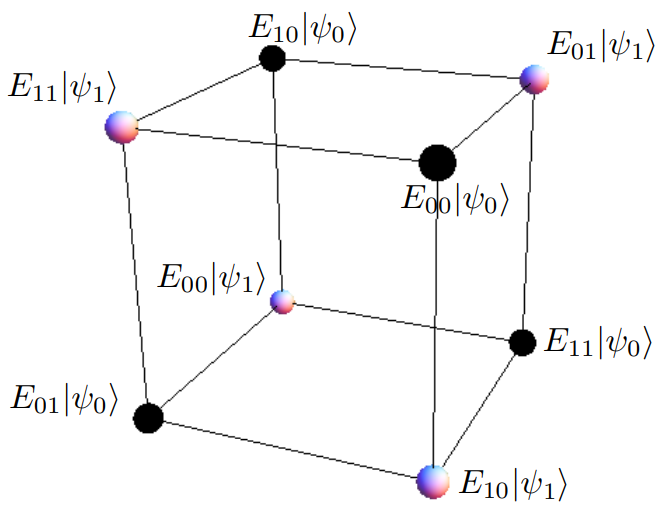
\includegraphics[width=0.5\linewidth]{Eightstatecube.png}
	\caption{A cube representing the eight cipherstates $E_{uw}\ket{\psi_{g}}$ as its corner points $(\pm1,\pm1,\pm1)^T/\sqrt{3}$ \cite{DeVries2016}.}
	\label{fig:eightstatecube}
	\end{center}
\end{figure}
\end{center}

We do not need to introduce much new notation or formalism for eight state encoding since we have essentially seen most of it already. The quantum one time pad is actually an eight state encryption protocol. The main difference is that in the protocol introduced for QKR, the eight states are distributed differently over the Bloch sphere. Diagrammatically, we can exploit the similarities by borrowing the notation that was previously introduced for the Pauli's in the QOTP. According to equation (\ref{equation:EightStatePaulis}), we only need to define one of the bases of eight state encoding and get the others for free by applying Pauli's to the states of this original basis. We choose the color red for this new basis. The red basis has the following two basis states: $E_{00}\ket{\psi_{0}} = \ket{\psi_{000}}$ and $E_{00}\ket{\psi_{1}} = \ket{\psi_{001}}$. We should first define triangles that represent classical information on these states, similarly to how we have classical triangles for the gray and white bases. We use the color red for this as well. This gives us the following diagrammatic components for the preparation of a state and the effect in this basis:

\begin{equation}
	\ket{\psi_{00g}} \equiv \tikzfig{RedStatePrep} ~~~~~~ \bra{\psi_{00g}} \equiv \tikzfig{RedEffect}
\end{equation}

Note that we have as well that:

\begin{equation}
\label{equation:RedMeasureAndEffect}
\tikzfig{PrepAndMeasureRed} \equiv \delta_{ij}
\end{equation}

Finally, we need to define a spider that encodes these $\ket{\psi_{000}}$ and $\ket{\psi_{001}}$ to the respective quantum states. In fact, since equation (\ref{equation:spidermultilegdecomposed}) is independent for the choice of basis, we can just copy it and exchange the white triangles for red ones:

\begin{equation}
	\label{equation:RedSpiderPrepareAndMeasure}
\tikzfig{spidermultilegred} = \tikzfig{spidermultilegdecomposedred}
\end{equation}

By a combination of equations (\ref{equation:RedMeasureAndEffect}) and (\ref{equation:RedSpiderPrepareAndMeasure}) it is trivial to check that the red spider follows the spider rules as they are given in section \ref{spiders}. With that being said, we have to tread carefully regarding its interaction with differently colored spiders, since we cannot exploit mutual unbiasedness.

We are now in principle ready to employ eight state encoding as it was proposed in \cite{DeVries2016} diagrammatically. Equation (\ref{equation:BellMap}) tells us how we can make Pauli's diagrammatically, and equation (\ref{equation:EightStatePaulis}) tells us that we can create all of our bases by applying these Pauli's to the recently defined new basis states $\ket{\psi_{00g}}$. We could thus encode all of our eight different cipherstates as follows:

\begin{equation}
	\label{equation:EightStateEncodingInFull}
	E_{uw}\ket{\psi_{00g}} \Leftrightarrow\tikzfig{EightStateEncodingInFullX}
\end{equation}

However, since the different bases will reappear quite often, we can save ourselves from unnecessarily complex diagrams by redefining each combination of $u$ and $w$ into a new spider, each with a different color. These eight state encoding spiders represent the four bases of eight state encoding in much the same way the gray and white spider represent the two bases of four state encoding.

%\footnote{Note that all four of these spiders accept red colored triangles because we defined all of them as Pauli's with respect to states in the red basis. The red basis has thus been given a privileged position among the four colors. This is in line with \cite{DeVries2016}, where the authors suggest to encode a classical '0' as $\ket{\psi_{000}}$ and a '1' as $\ket{\psi_{001}}$, and define the other states as Pauli's with respect to these.} 

\begin{equation}
	\label{equation:EncryptionOperators}
	\{u,w\} = \{0, 0\} \Leftrightarrow \tikzfig{RedEncoding} ~~~~~~ \{u,w\} = \{0, 1\} \Leftrightarrow \tikzfig{YellowEncoding}~~~~~~ \{u,w\} = \{1, 0\} \Leftrightarrow \tikzfig{GreenEncoding}~~~~~~ \{u,w\} = \{1, 1\} \Leftrightarrow \tikzfig{BlueEncoding}
\end{equation}

Finally, to make our lives easier, we introduce one more spider. This spider is actually nothing new, it is the set of the four spiders introduced in \ref{equation:EncryptionOperators}. Having this spider may come in handy whenever we want to make a statement that counts for all four of the colored spiders. Instead of making the same statement for each of the different spiders, we can then make it once for this new spider. We choose the color brown for this:

\begin{equation}
\label{equation:brownspiderset}
\tikzfig{BrownSpider} \equiv \{~\tikzfig{RedSpider},~ \tikzfig{GreenSpider},~ \tikzfig{OrangeSpider},~ \tikzfig{BlueSpider}\}
\end{equation}

Let's first see what our QKR protocol looks like in this new notation:

\begin{equation}
	\label{equation:QKRGeneralFirstIntroduced}
	\tikzfig{QKRGeneralX}
\end{equation}

Alice and Bob respectively encode and measure in the same basis. Eve controls some map $\Phi$ and receives one of its outputs. With this all set up we are in principle ready to develop a security proof for noiseless QKR, purely diagrammatically. Our security proof is very similar to the one proposed by Kissinger and Westerbaan in literature \cite{Kissinger2017}, where they prove security of four state QKD relying largely on the mutual unbiasedness of the gray and white bases. Although we do bring this mutual unbiasedness indirectly into our security proof as well by incorporating the Pauli's consistent of the gray and white spiders that we have seen before, we aim to extend this proof to also incorporate our four new non-mutually unbiased bases. As we will see, we will rely on gray and white spiders only through the use of these Pauli's, which are a valid member of eight state encoding.

Putting in the property that the quantum channels and maps exhibit no noise according to Alice and Bob is equivalent to saying that Eve goes undetected whenever Alice and Bob measure in the same basis. Since Eve represents the environment this can also be interpreted as the quantum channels being noiseless. We have already briefly discussed the security proof of Kissinger and Westerbaan in section \ref{QuantumKeyDistribution}, where we made the same statement for Alice and Bob using the gray and white bases. Noting that brown represents the set of four colors introduced in equation (\ref{equation:brownspiderset}), we can implement this statement for our four new bases as follows:

\begin{equation}
	\label{equation:coloredspiders}
	\tikzfig{QKRProofSetupX} = \tikzfig{wire} ~~~~ \land ~~~~ \tikzfig{QKRProofSetupGreenX} = \tikzfig{wire} ~~~~ \land ~~~~ \tikzfig{QKRProofSetupYellowX} = \tikzfig{wire} ~~~~ \land ~~~~ \tikzfig{QKRProofSetupBlueX} = \tikzfig{wire} ~~~~ \Leftrightarrow ~~~~ \tikzfig{QAaSBProofSetupReal1X} = 
\tikzfig{wire}
\end{equation}

With this as a starting point we can pre- and postcompose measurement maps as follows:

\begin{equation}
	\label{equation:QKDSetupRed}
	\tikzfig{QKDProof1X} = \tikzfig{QKDProof2}
\end{equation}

Now we can purify the brown spiders in equation (\ref{equation:QKDSetupRed}) by doubling and discarding an extra output according to equation (\ref{equation:Purification}). Note that we can also, without loss of generality, state that $\Phi = \hat{V}$ since $\Phi$ already fits the definition of a purified state given in section \ref{discarding}. This gives rise to the following diagrams:

\begin{equation}
	\label{equation:QKRProof4}
	\tikzfig{QKRProof4X} = \tikzfig{QKRProof4AX} \equaltext{(\ref{equation:discarding})} \tikzfig{QKRProof5X}
\end{equation}
\textit{Where $\hat{\psi}$ can be any normalized pure state.}

By applying the essential uniqueness of purification from section \ref{section:essentialuniqueness} to equation \ref{equation:QKRProof4} we get to equation (\ref{equation:PurifiedQKR}). Note that since we discarded multiple outputs in equation (\ref{equation:QKRProof4}) we also have to apply the unitary U multiple outputs:

\begin{equation}
	\label{equation:PurifiedQKR}
	\tikzfig{QKRProof6X} = \tikzfig{QKRProof7X}
\end{equation}

Deleting the second and fourth output of the LHS of equation (\ref{equation:PurifiedQKR}) gives the following:

\begin{equation}
	\tikzfig{QKRProof6AX} \equaltext{\ref{spiders}} \tikzfig{QKRProof6BX}
\end{equation}

Doing the same to the RHS of equation (\ref{equation:PurifiedQKR}):

\begin{equation}
	\label{equation:passingvonthrough}
	 \tikzfig{QKRProof6BX} = \tikzfig{QKRProof9X}
\end{equation}

Note that this holds for spiders of all colors of equation (\ref{equation:coloredspiders}). The following is thus also true for spiders of all these colors:

\begin{equation}
\label{equation:vrules}
	\tikzfig{QKRProof10X} \equaltext{(\ref{equation:passingvonthrough}), \ref{spiders}} \tikzfig{QKRProof11X} ~~~~~~~~~~~~~~~~~~ \tikzfig{QKRProof12X} \equaltext{(\ref{equation:passingvonthrough}), \ref{spiders}} \tikzfig{QKRProof13X}
\end{equation}

Using equation (\ref{equation:vrules}) we can prove that V separates. Starting with V itself:

\begin{equation}
	\label{equation:v}
	\tikzfig{QKRSeperationProof1X}
\end{equation}

The strategy is to add something separated from the diagram in equation (\ref{equation:v}) and put V in there. We can just compose the creation and deletion of a random variable. Adding it to the diagram and writing one output of V a bit more suggestively:

\begin{equation}
	\label{equation:vwithpauli}
	(\ref{equation:v}) \equaltext{\ref{spiders}} \frac{1}{D}~
	\tikzfig{QKRSeperationProof2X}
\end{equation}

Now, we need some method to attach the separated part to the diagram temporarily such that we can move V through. It turns out that eight state encoding gives us a map that can do exactly this: the random Pauli's. Equation (\ref{equation:AliceWithBell}) already showed how a random Pauli can separate two parts of a diagram. We place it between the two diagrams in equation (\ref{equation:vwithpauli}):

\begin{equation}
(\ref{equation:vwithpauli}) \equaltext{(\ref{equation:AliceWithBell})} \tikzfig{QKRSeperationProof3X} \equaltext{(\ref{equation:vrules})} \tikzfig{QKRSeperationProof4X}
\end{equation}

What we need now is some way to pass V through this Pauli. Isolating just the Pauli and the encoding map:

\begin{equation}
	\label{equation:RedSpiderRandomPauli}
	\tikzfig{QKRSeperationProof5X}
\end{equation}

So what we have here is a random Pauli, precomposed by any of the four encoding maps. Since each of the four bases are just Pauli's with respect to one another, combining the encoding and random Pauli maps actually selects one of the four bases to encode in at random. More explicitly, remember by equation (\ref{equation:EightStatePaulis}) that each of the cipherstates can be created by two Pauli's and the $\ket{\psi_g}$ basis states ($\ket{\psi_{uwg}} = X^w Z^u\ket{\psi_{g}}$). Then applying a random Pauli ($X^n Z^m~where~n~and~m~are~random$) to any of the cipherstates gives the following:

\begin{equation}
\label{equation:EncodingInRandomCipherstate}
X^nZ^mX^uZ^w\ket{\psi_{g}} = X^lZ^p\ket{\psi_{g}} \equaltext{\ref{equation:EightStatePaulis}} \ket{\psi_{lpg}} ~(\text{where}~ l \equiv n \oplus u ~\text{and}~ p \equiv m \oplus w)
\end{equation}

Which, by randomness of $l$ and $p$, is a cipherstate encoded into a random one of the bases. Encoding a state into a cipherstate with a certain basis and then applying a random Pauli is thus equivalent to encoding this cipherstate into a random basis. We can find this diagrammatically too. Remember that equation (\ref{equation:EightStateEncodingInFull}) tells us how we can encode any state with respect to the red basis by applying two Pauli's diagrammatically. The brown spider that is used for encoding in equation (\ref{equation:RedSpiderRandomPauli}) can thus be replaced by a red spider and two Pauli's.\footnote{The careful reader may notice that replacing the brown encoding spider in equation (\ref{equation:RedSpiderRandomPauli}) by a red encoding spider and two subsequent Pauli's brings with it some further complications. This is because the red encoding spider accepts classical data only in the red basis, whereas the brown spider could accept all the colors of classical data. In this section, this will not form a problem. Since we do not do any classical processing on the data, we could just assume all the classical data is encoded into the red basis. In section \ref{section:QAaSBEequivalences}, where we will mix classical processing with colored spiders, we define a map that can solve this issue accordingly.} Looking just at this encoding part and the random Pauli's that follow immediately after we thus get:

\begin{equation}
	\label{equation:composingtwopaulis}
 \tikzfig{ComposingTwoPauli's}
\end{equation}

The only ingredient that we are missing is some way to move Pauli's past one another. Mathematically, the fact that we can do this is evident from the anticommutative property of Pauli's. Anticommutativity implies that any two Pauli's $\sigma_i$ and $\sigma_j$ satisfy $\sigma_i\sigma_j = - \sigma_j\sigma_i$. Diagrammatically we can commute Pauli's using the $k-k'$ commute rule from section \ref{section:kkcommute} as follows:

\begin{equation}
\label{equation:commutingpaulis}
\tikzfig{CommutingPauli's} \equaltext{\ref{equation:RandomXBitFlipProof}} \tikzfig{CommutingPauli's1} \equaltext{\ref{equation:kkcommuterule}} \tikzfig{commutingPauli's3} \equaltext{\ref{equation:RandomXBitFlipProof}} \tikzfig{CommutingPauli's4}
\end{equation}

Putting this back into equation \ref{equation:composingtwopaulis} and moving around some spiders gives:

\begin{equation}
	(\ref{equation:composingtwopaulis}) \equaltext{\ref{equation:spidermultilegdecomposed}} \sum\limits_{nm}\tikzfig{ComposingTwoPauli's2} \equaltext{\ref{equation:commutingpaulis}}
	\sum\limits_{nm}\tikzfig{ComposingTwoPauli's3} \equaltext{\ref{equation:spiderfusion}}
	\sum\limits_{nm}\tikzfig{ComposingTwoPauli's4}
	\equaltext{\ref{equation:spiderfusion}}
	\sum\limits_{nm}\tikzfig{ComposingTwoPauli's5}
\end{equation}

By equation (\ref{equation:xormap}) we know that the m and w here are xor'd by the gray spider and the n and u are xor'd by the white spider. We define $m \oplus w \equiv p$ and $n \oplus u \equiv l$, where randomness of m and n implies randomness of p and l. This gives:

\begin{equation}
	\sum\limits_{lp} \tikzfig{ComposingTwoPauli's6}
\end{equation}

Which is by itself encoding into a random basis by equation (\ref{equation:EightStateEncodingInFull}). Putting this back into equation \ref{equation:RedSpiderRandomPauli}:
%Incorporating (\ref{equation:EncodingInRandomCipherstate}) into equation (\ref{equation:RedSpiderRandomPauli}) we get the following:

\begin{equation}
	\label{equation:fourcolourspiders}
	(\ref{equation:RedSpiderRandomPauli}) \equaltext{\ref{equation:EncodingInRandomCipherstate}} \frac{1}{4}\tikzfig{QKRSeperationProof7} + \frac{1}{4} \tikzfig{QKRSeperationProof7B} + \frac{1}{4} \tikzfig{QKRSeperationProof7C} + \frac{1}{4} \tikzfig{QKRSeperationProof7D}
\end{equation}

By undoubling the wire in the middle and using equation (\ref{equation:vrules}) we can move V through all of these:

\begin{equation}
\label{equation:passingvthroughpauli}
\begin{aligned}
	 \tikzfig{QKRSeperationProof8X} \equaltext{(\ref{equation:fourcolourspiders})} \frac{1}{4}\tikzfig{QKRSeperationProof9AX} + \frac{1}{4} \tikzfig{QKRSeperationProof9BX} + \frac{1}{4} \tikzfig{QKRSeperationProof9CX} + \frac{1}{4} \tikzfig{QKRSeperationProof9DX} \\ \equaltext{(\ref{equation:vrules})}
	 \frac{1}{4}\tikzfig{QKRSeperationProof9BAX} + \frac{1}{4} \tikzfig{QKRSeperationProof9BBX} + \frac{1}{4} \tikzfig{QKRSeperationProof9BCX} + \frac{1}{4} \tikzfig{QKRSeperationProof9BDX} \\
	 \equaltext{(\ref{equation:vrules})}
	  \frac{1}{4}\tikzfig{QKRSeperationProof10AX} + \frac{1}{4} \tikzfig{QKRSeperationProof10BX} + \frac{1}{4} \tikzfig{QKRSeperationProof10CX} + \frac{1}{4} \tikzfig{QKRSeperationProof10DX} \equaltext{(\ref{equation:fourcolourspiders})} \tikzfig{QKRSeperationProof11X}
\end{aligned}
\end{equation}

Putting this back into the larger picture:

\begin{equation}
	\label{equation:vpassingthrough}
	\tikzfig{QKRSeperationProof4X} \equaltext{(\ref{equation:passingvthroughpauli})} \frac{1}{D}~ \tikzfig{QKRSeperationProof12X} \equaltext{(\ref{equation:AliceWithBell})}	\frac{1}{D}~ \tikzfig{QKRSeperationProof13X} \equaltext{\ref{spiders}} \frac{1}{D}~ \tikzfig{QKRSeperationProof14X}
\end{equation}

And thus we see that V separates. Hence, under the condition that Alice and Bob measure and encode in the same four bases from equation (\ref{equation:brownspiderset}), $\Phi$ separates. In diagrams:

\begin{equation}
\label{equation:QKRSeparates}
\tikzfig{QKRSeperationProof15X} = \tikzfig{QKRSeperationProof16X}
\end{equation}

\section{Equivalences}
\label{Equivalences}

\subsection{QOTP and Quantum Teleportation}

The equivalence of QOTP and quantum teleportation is rather trivial. In fact, we already saw this equivalence back in equation (\ref{equation:QOTPQuantumTeleportationEquivalence}):

\begin{equation}
\tikzfig{QOTPNoEveNoLineX} \equaltext{\ref{spiders}} \tikzfig{QOTPNoEveNoLine(1)}~~~~~ \Leftrightarrow ~~~~~\tikzfig{QuantumTeleportationNoLine}
\end{equation}

This is a strikingly simple equivalence. Bending the U-shaped curve in the quantum teleportation protocol such that it becomes a straight line already does the trick. In a sense, quantum teleportation could thus be seen as the EPR variant of the QOTP. 

Due to their equivalence, whatever we can prove with the one diagram we can state as fact for the other without needing to prove it. This can be very convenient in security proofs.

\subsection{QKD Prepare and Measure and QKD EPR}

In the introduction we discussed the

\subsection{Quantum Alice and Silent Bob Equivalences}

\label{section:QAaSBEequivalences}
In a recent article \cite{Leermakers2019}, Skori$\check{\textrm{c}}$ and Leermakers propose a scheme for QKR that includes no classical communication from Alice to Bob and only one bit from Bob to Alice. To prove its security, the authors modify the proposed protocol to one that is better suited for this in a series of steps that preserve security-wise equivalence to the original. In this section, we will have a look at these equivalences diagrammatically using the eight state encoding QKR protocol from equation (\ref{equation:QKRGeneral}) as starting point:

\begin{equation}
\label{equation:QKRGeneral}
	\tikzfig{QKRGeneralX}
\end{equation}


\subsubsection{Masking the qubit payload with public randomness}
\label{section:maskingqubitpubrand}
In the first equivalent protocol Alice and Bob both apply the same bitstring $a \in \{0,1\}^n$ in the classical domain, before encoding and after decoding respectively. $a$ is public, implying that Eve also learns it. The rest of the protocol remains the same. To implement this diagrammatically, we give Eve another map with respect to (\ref{equation:EveNewMap}) to represent her doing classical post processing. In this map, she uses her knowledge on $a$ and what she learned from intercepting the quantum state from Alice to Bob.

We need to create one more set of maps before we can implement this diagrammatically. Since we haven't fully worked out all of the properties of the colored spiders yet, it is more convenient to not use them whenever the protocol doesn't tell us to. Therefore, we propose a map that translates between the white and colored bases. This allows us to do all of the classical processing in terms of white and gray spiders which is necessary if we want to use for example mutual unbiasedness (\ref{complementarity}) or the xor map (\ref{xorgate}). The map that translates between the white and red bases is the following:

\begin{equation}
\label{equation:EightStateSpider}
\tikzfig{EightStateSpider} :
\ket{g}_z \mapsto \ket{\psi_{00g}} ~~~~ \tikzfig{REightStateSpider} :
\ket{\psi_{00g}} \mapsto \ket{g}_z
\end{equation}

This map is worked out in Dirac notation in appendix \ref{}. The other three colors then also have the respective boxes:

\begin{equation}
\label{equation:EightStateSpiderGreen}
\tikzfig{EightStateSpiderGreen} :
\ket{g}_z \mapsto \ket{\psi_{10g}} ~~~~ \tikzfig{REightStateSpiderGreen} :
\ket{\psi_{10g}} \mapsto \ket{g}_z
\end{equation}

\begin{equation}
\label{equation:EightStateSpiderOrange}
\tikzfig{EightStateSpiderOrange} :
\ket{g}_z \mapsto \ket{\psi_{01g}} ~~~~ \tikzfig{REightStateSpiderOrange} :
\ket{\psi_{01g}} \mapsto \ket{g}_z
\end{equation}

\begin{equation}
\label{equation:EightStateSpiderBlue}
\tikzfig{EightStateSpiderBlue} :
\ket{g}_z \mapsto \ket{\psi_{11g}} ~~~~ \tikzfig{REightStateSpiderBlue} :
\ket{\psi_{11g}} \mapsto \ket{g}_z
\end{equation}

We call these maps the eight state encryption maps. Again, the brown box is the set of the four individual maps:

\begin{equation}
	\label{brownbox}
	\tikzfig{EightStateSpiderBrown} \equiv \{ ~\tikzfig{EightStateSpider}, ~\tikzfig{EightStateSpiderGreen}, ~\tikzfig{EightStateSpiderOrange}, ~\tikzfig{EightStateSpiderBlue}\}
	~~~~~~~~~
	\tikzfig{REightStateSpiderBrown} \equiv \{ ~\tikzfig{REightStateSpider}, ~\tikzfig{REightStateSpiderGreen}, ~\tikzfig{REightStateSpiderOrange}, ~\tikzfig{REightStateSpiderBlue}\}
\end{equation}

Including this map, and the fact that Alice and Bob both xor with a public variable $a$ in their classical domain, we have the following diagram:

\begin{equation}
	\label{equation:QKRQAaSBA1}
	\tikzfig{QKRQAaSBA1X}
\end{equation}
\textit{With $\Phi_1$ the map that Eve uses to intercept the communication and $\Phi_2$ the map that Eve uses to do classical processing on both this intercepted data and $a$.}

%The central part of this diagram - Eve's map $\Phi_1$ and the %encoding and measuring operations by Alice and Bob - we have already %seen (\ref{equation:coloredspiders}). This is the QKR protocol which %we have proven secure in section \ref{section:qkr}.
For a security proof of this protocol, we can state that Eve's operations introduce no noise from Alice and Bob's perspective whenever they measure in the same basis. This is the same statement that we made in section \ref{section:qkr} to prove the security of QKR, and in section \ref{QuantumKeyDistribution} to prove the security of QKD.For the diagram in equation (\ref{equation:QKRQAaSBA1}), this looks as follows:

\begin{equation}
\label{equation:QAaSBProofSetupReal}
\tikzfig{QKRQAaSBA1DiscardingEveX} = ~~ \tikzfig{longwire}
\end{equation}

By causality we then know that applying Eve's map $\Phi_2$ and then deleting the output is essentially the same as not having applied Eve's map altogether:

\begin{equation}
\label{equation:QKRQAaSBA1DiscardingEve1}
\tikzfig{QKRQAaSBA1DiscardingEve1X} = ~~ \tikzfig{longwire}
~~\Leftrightarrow
\tikzfig{QKRQAaSBA1DiscardingEve2X} = ~~ \tikzfig{longwire}
\end{equation}

Then we can pre and postcompose another xor with $a$ on both sides of equation (\ref{equation:QKRQAaSBA1DiscardingEve1}):

\begin{equation}\\
\label{equation:QKRQAaSBA1DiscardingEve3}
\tikzfig{QKRQAaSBA1DiscardingEve3X} = ~~ \tikzfig{longwire1X} ~
\Leftrightarrow
\tikzfig{QKRQAaSBA1DiscardingEve4X} = ~~ \tikzfig{longwire2X}
\end{equation}

According to the diagrammatic rules for mutual unbiasedness given in equation (\ref{equation:Complementarity}) this separates $a$ on both sides of equation (\ref{equation:QKRQAaSBA1DiscardingEve1}):

\begin{equation}
\label{QKRQAaSBA1DiscardingEve5}
\tikzfig{QKRQAaSBA1DiscardingEve5X} = ~~ \tikzfig{longwire3X}
\end{equation}

Which is up to a constant factor equivalent to the same diagrams without a random $a$:

\begin{equation}
\tikzfig{QKRQAaSBA1DiscardingEve6X} = ~~ \tikzfig{longwire4} ~~ = ~~ \tikzfig{longwire}
\end{equation}

Finally, by exploiting unitarity of the brown eight state encoding map we get the following:

\begin{equation}
\tikzfig{QKRQAaSBA1DiscardingEve8X} = ~~ \tikzfig{longwire5} ~ \Leftrightarrow ~~ \tikzfig{QKRQAaSBA1DiscardingEve9X} = ~~ \tikzfig{wire}
\end{equation}


This equation we have already seen, it is the starting point for the security proof of eight state encoding QKR (equation (\ref{equation:QKDSetupRed})).\footnote{There is of course a minor difference: In (\ref{equation:QKDSetupRed}) Eve has the map $\Phi$ and here Eve has the map $\Phi_1$. This is insignificant however. $\Phi_1$ was only introduced to distinguish between Eve's quantum map and Eve's classical map. We can just say that $\Phi$ = $\Phi_1$ without loss of generality since Eve's quantum map can be any (multitude of) unspecified operation(s) in both cases.} Therefore, we could just follow all the steps which we followed in section \ref{section:qkr} and get as a result that $\Phi_1$ separates as follows:\footnote{This is also why they are security-wise equivalent, they follow the same security proof. If it turns out that the security proof in section \ref{section:qkr} for the original QKR protocol only allows for security up to some factor, the protocol with public randomness from this section is also only secure up to that same factor.}

\begin{equation}
	\label{equation:QKRGeneralSeparation}
	\tikzfig{QKRGeneralQAaSBNoMeasuringX} = \tikzfig{QKRGeneralQAaSBSeparatedX}
\end{equation}

Putting this back into equation (\ref{equation:QKRQAaSBA1}) we get the following:

\begin{equation}
	\tikzfig{QKRQAaSBA1NoDottedLineX} \equaltext{\ref{equation:QKRGeneralSeparation}} \tikzfig{QKRQAaSBA2X}
\end{equation}

In a series of steps following rules which we have seen before we can show that Eve's map again separates entirely from Alice and Bob's part of the diagram:

\begin{equation}
	\begin{aligned}
	\tikzfig{QKRQAaSBA3X} \equaltext{\ref{equation:EightStateSpider}} \tikzfig{QKRQAaSBA4X} \equaltext{\ref{equation:spiderfusion}} \tikzfig{QKRQAaSBA5X} \\ \equaltext{\ref{doubling}} \tikzfig{QKRQAaSBA6X} \equaltext{\ref{equation:Complementarity}} \tikzfig{QKRQaASBA7X} = \tikzfig{QKRQAaSBA8X}
	\end{aligned}
\end{equation}

So we see that even though Eve gets $a$ and some quantum state, she is not attached to Alice and Bob's communication channel. Alice and Bob on the other hand achieve uninterrupted communication. This is what we would intuitively expect for the noiseless case.

\subsubsection{EPR version of the protocol}

\label{section:eprqkr}
The second equivalent protocol is an EPR version of the original. We have already seen a diagrammatic implementation of an EPR protocol in section \ref{subsection:QuantumTeleportation}, the diagram for quantum teleportation. The characteristic difference between an EPR version of a protocol and a normal version is that in the former Alice and Bob share some entangled qubit. In quantum teleportation this is the Bell state, given by the doubled wire shaped like a cup in equation (\ref{quantumteleportation}).

Diagrammatically, it is rather trivial to go from the protocol introduced in the previous section (\ref{equation:QKRQAaSBA1}) to an EPR version. In fact, we only need to bend around some wires. We split this up in a few steps to show where all the parts go. First of all, bending around Alice's wire according to the yanking equation (\ref{equation:yankingequation}):

\begin{equation}
	\label{equation:QAaSBEPREquivalence}
	\begin{aligned}
	\tikzfig{QKRQAaSBA1NoDottedLineX} \equaltext{\ref{equation:yankingequation}} \tikzfig{QKRQAaSBB2X}
	\end{aligned}
\end{equation}

And subsequently pulling her encoding and encryption operations through:

\begin{equation}
\label{equation:EPRQKR}
	\begin{aligned}
 (\ref{equation:QAaSBEPREquivalence}) = \tikzfig{QKRQAaSBB3X} = \tikzfig{QKRQAaSBB4DottedLineX}
\end{aligned}
\end{equation}

Which is indeed the EPR version of the protocol in equation (\ref{equation:QKRQAaSBA1}): 

\begin{equation}
\label{equation:QKRQAaSBB4DottedLine}
	(\ref{equation:QAaSBEPREquivalence}) = \tikzfig{QKRQAaSBB4DottedLineX} \Leftrightarrow \tikzfig{QKRQAaSBA1X} = (\ref{equation:QKRQAaSBA1})
\end{equation}

Of course, if these protocols are equivalent, then by security-wise equivalence of (\ref{equation:QKRQAaSBA1}) and (\ref{equation:QKRGeneral}) we also have security-wise equivalence of the EPR version introduced in this section, (\ref{equation:QAaSBEPREquivalence}), and (\ref{equation:QKRGeneral}). 

\subsubsection{Adding a random permutation}

In the next equivalent step, the authors propose that Alice and Bob both publicly decide on the same random permutation ($\pi$) to apply to their own set of qubit states before measuring, and forget it right after. Eve, however, can remember this $\pi$. Diagrammatically, this looks as follows:

\begin{equation}
	\label{equation:QKRQAaSBC1}
	\tikzfig{QKRQAaSBC1X}
\end{equation}

Intuitively, it is evident that this step preserves equivalence to the original from Alice and Bob's perspective due to the fact that this steps preserves entanglement of the EPR states. Whether this protocol works or not for Alice and Bob is independent on the choice of states that they receive, as long as they are entangled. The states that Eve sends to Alice and Bob are entangled up to a certain degree dependent on the amount of noise Eve introduces, and the $\pi$'s completely preserve entanglement since the same operation is applied on both qubits. To make a diagrammatic proof from this intuition we have to first exploit the fact that we can turn Eve's map into a state. We can do this as follows:

\begin{equation}
\label{equation:QKRQAaSBC6}
\tikzfig{QKRQAaSBC1X} = \tikzfig{QKRQAaSBC6X}
\end{equation}
\textit{Note that the dotted map in this diagram has no diagrammatic significance and is only intended for didactic purposes}

We can show that this is a valid operation diagrammatically. Isolating just the state of Eve in the RHS of equation (\ref{equation:QKRQAaSBC6}) and realizing that Eve has the freedom to do whatever she wants in her state $\Phi_1$:

\begin{equation}
\label{equation:QKRQAaSBC7}
\tikzfig{QKRQAaSBC7} = \tikzfig{QKRQAaSBC8}
\end{equation}

Then using the yanking equation (\ref{equation:yankingequation}):

\begin{equation}
\label{equation:QKRQAaSBC9}
(\ref{equation:QKRQAaSBC7}) = \tikzfig{QKRQAaSBC9} \equaltext{\ref{equation:yankingequation}} \tikzfig{QKRQAaSBC10}
\end{equation}

We see that we can transform Eve's map into a state and reversedly. The operation from equation (\ref{equation:QKRQAaSBC6}) is therefore valid.

Starting with the RHS of equation (\ref{equation:QKRQAaSBC6}) and using the yanking equation (\ref{equation:yankingequation}):

\begin{equation}
\begin{aligned}
\label{equation:QKRQAaSBC11}
 (\ref{equation:QKRQAaSBC6}) = \tikzfig{QKRQAaSBC11X} \equaltext{\ref{equation:yankingequation}} \tikzfig{QKRQAaSBC12X}
\end{aligned}
\end{equation}

Now we are ready to put in the intuition that we had in the beginning of this section. From Alice and Bob's perspective, everything they need is for Eve to prepare and send them an (imperfect) EPR state. If Eve does this in her map $\Phi_1$ the two subsequent random permutations will potentially change the particular choice of EPR states that Alice and Bob receive, but they will remain entangled since the same operation is applied on both sides. Furthermore, Alice and Bob forget $\pi$ right after they apply it. For Eve, 

\begin{equation}
	\label{equation:QKRQAaSBC13}
	(\ref{equation:QKRQAaSBC11}) = \tikzfig{QKRQAaSBC12AX} = \tikzfig{QKRQAaSBC13X}
\end{equation}

\subsubsection{Adding random Pauli transforms}

In the final equivalent step, the authors propose that Alice and Bob both publicly decide on the same random Pauli to apply to their own qubit states before measuring. Afterwards they again forget the particular choice of Pauli. Diagrammatically, this looks as follows: 

\begin{equation}
\label{equation:QKRQAaSBD1}
\tikzfig{QKRQAaSBD1X}
\end{equation}

The difference between this protocol and the EPR protocol introduced in section \ref{section:eprqkr} are the two single spiders in the middle which represent the classical random variables that determine the Pauli's which are applied to both Alice and Bob's states. Information on the particular choice of Pauli's also goes to Eve by the thin lines originating from these two single spiders. Let's isolate the Pauli that Alice gets and her measurement and eight state encryption maps:

\begin{equation}
	\label{equation:QKRPauli's}
	\tikzfig{QKRPauli's1X} \Rightarrow \tikzfig{QKRPauli's2} = \sum\limits_{nm} \tikzfig{QKRPauli's3}  = \sum\limits_{nm} \tikzfig{QKRPauli's4}
\end{equation}

We do not consider the two triangles that go to Bob for now. These simply determine the Pauli's that he applies to his qubit state. All we need to know is that they are the same as Alice's. Furthermore we can take the brown decoding spider of Alice further apart according to equation (\ref{equation:EightStateEncodingInFull}). This equation shows how all the cipherstates can be encoded by a red spider and two Pauli's. Since decoding is the adjoint of decoding, we can decode in any of the four bases by first applying two Pauli's followed by a red spider. To then return back to the classical z basis we need to also exchange the brown eight state encryption box for a red one:

\begin{equation}
	\label{equation:QKRQAaSBD3}
	(\ref{equation:QKRPauli's}) = \sum\limits_{nm}\tikzfig{QKRQAaSBD3}
\end{equation}

This equation is very similar to equation (\ref{equation:composingtwopaulis}). In fact, for equation (\ref{equation:composingtwopaulis}) we showed that encoding in a certain basis and then applying a random Pauli results in encoding in a random basis. Here we will show that applying a random Pauli and then decoding in a certain basis results in decoding in a random basis: \footnote{The main differences between equations (\ref{equation:composingtwopaulis}) and (\ref{equation:QKRQAaSBD3}) are that in the latter we send some information to Eve and use the eight state encryption map. Sending some information to Eve will play an important role later. The fact that we do not use the eight state encryption map in equation (\ref{equation:composingtwopaulis}) is actually not that big of a difference. In fact, we could have added it in there already, it was just not necessary. Adding it in helps us translate between the four bases of eight state encoding and the z basis such that we can do classical processing in the basis for which we have defined the relevant tools, such as the xor map. Since back in equation (\ref{equation:composingtwopaulis}) we did not do such classical processing introducing this map was unnecessary.} 

\begin{equation}
\label{equation:QKRQAaSBD4}
(\ref{equation:QKRQAaSBD3}) \equaltext{\ref{equation:commutingpaulis}} \sum\limits_{nm}\tikzfig{QKRQAaSBD4} \equaltext{\ref{equation:spiderfusion}} \sum\limits_{nm}\tikzfig{QKRQAaSBD5} \equaltext{\ref{equation:spiderfusion}} \sum\limits_{nm}\tikzfig{QKRQAaSBD6} 
\end{equation}

By equation (\ref{equation:xormap}) we know that the gray n and u are xor'd by the white spider and that the white m and w are xor'd by the gray spider. Defining $m \oplus w \equiv p$ and $n \oplus u \equiv l$ and realizing that l and p are random then gives: 

\begin{equation}
	\label{equation:randompaulidecoding}
	(\ref{equation:QKRQAaSBD4}) = 
	\sum\limits_{nmlp}\tikzfig{QKRQAaSBD7} = \sum\limits_{lp}\tikzfig{QKRQAaSBD8}
\end{equation}

As expected, Eve receives the random variables n and m, but she does not learn l and p since these require knowledge of u and w. Alice and Bob thus measure in a random basis and Eve doesn't know this basis. More importantly for Alice and Bob, they measure in the same random basis since for Bob's side, the whole derivation follows the same series of steps. Putting this back into the larger picture, equation (\ref{equation:QKRQAaSBD1}):

\begin{equation}
	\label{equation:QKRQAaSBDResult}
	\begin{aligned}
	(\ref{equation:QKRQAaSBD1}) \equaltext{\ref{equation:randompaulidecoding}}
	\sum\limits_{lp}\tikzfig{QKRQAaSBD12} = \frac{1}{4}\tikzfig{QKRQAaSBDResultR} \\+
	\frac{1}{4}\tikzfig{QKRQAaSBDResultG} +
	\frac{1}{4}\tikzfig{QKRQAaSBDResultO} +
	\frac{1}{4}\tikzfig{QKRQAaSBDResultB}
	\end{aligned}
\end{equation}

Each of these protocols occur with probability $\frac{1}{4}$. We also know that they are all security-wise equivalent to the protocol in equation (\ref{equation:EPRQKR}) since they form the members of the set of protocols in the RHS of equation \ref{equation:EPRQKR}. The protocol in equation (\ref{equation:QKRQAaSBD1}) thus preserves security-wise equivalence to the protocol that was the starting point of this section, equation (\ref{equation:QKRGeneral}).

\bibliographystyle{plain}
\bibliography{library}
\appendix


\section{Keywords}
\label{Keywords}


~~~~\hyperref[coloursandbases]{Base: E, page 2}

\hyperref[braandket]{Bra: A, page 1}

\hyperref[coloursandbases]{Colour: E, page 2}

\hyperref[phasespiders]{Decoding: H, page 3}

\hyperref[discarding]{Density matrix: G, page 3}

\hyperref[discarding]{Discarding:G, page 3}

\hyperref[doubling]{Doubling: F, page 2}

\hyperref[braandket]{Effect: A, page 1}

\hyperref[braandket]{Hermitian Adjoint: A, page 1}

\hyperref[braandket]{Hermitian Conjugate: A, page 1}

\hyperref[identity]{Identity: B, page 1}

\hyperref[braandket]{Ket: A, page 1}

\hyperref[spiders]{Kronecker delta: D, page 2}

\hyperref[maps]{Linear map: C, page 1}

\hyperref[phasespiders]{Phase: H, page 3}

\hyperref[phasespiders]{Phase spider: H, page 3}

\hyperref[doubling]{Purity: F and G, pages 2 and 3}

\hyperref[spiders]{Spider: D, page 2}

\hyperref[braandket]{State: A, page 1}

\hyperref[identity]{System type: B, page 1}

\hyperref[doubling]{Tensor product: F, page 3}

\hyperref[discarding]{Trace: G, page 3}

\hyperref[maps]{Map: C, page 1}

\hyperref[doubling]{Mixed state: F, page 2}

\hyperref[braandket]{Transpose: A, page 1}

\hyperref[identity]{Wire: B, page 1}

\section{Eight state encryption map in Dirac notation}
\label{appendix:EightStateEncryptionMapDirac}
Here we will work out the eight state encryption map in Dirac notation. This will reveal also the reasoning behind its shape. 

\begin{equation}
\tikzfig{EightStateSpiderBrown} :
\ket{g}_z \mapsto \ket{\psi_{uwg}}
\end{equation}

The operator that corresponds to this map, $G_{uw}$, is the following:

\begin{equation}
	G_{uw} \equiv \ket{0}_z\bra{\psi_{uw0}} + \ket{1}_z\bra{\psi_{uw1}}
\end{equation}

With its hermitian adjoint:

\begin{equation}
G_{uw}^\dagger \equiv \ket{\psi_{uw0}}\bra{0}_z + \ket{\psi_{uw1}}\bra{1}_z
\end{equation}

Corresponding to the following map:

\begin{equation}
\tikzfig{REightStateSpiderBrown} :
\ket{g}_z \mapsto \ket{\psi_{uwg}}
\end{equation}

Since $G_{uw} \neq G_{uw}^\dagger$ it is not self-adjoint and due to the complex elements in $\ket{\psi_{uwg}}$ it is not self-conjugate either. We do however know that it is unitary:

\begin{equation}
	G_{uw}G_{uw}^\dagger = \ket{0}_z\bra{0}_z + \ket{1}_z\bra{1}_z = \mathbb{1} \Leftrightarrow \tikzfig{UnitarySmllBrownBox} = \tikzfig{wire}
\end{equation}


\end{document}
